\section{Nonmonotonic Rule Learning}\label{sec:nmrulelearn}
So far we have considered approaches for constructing Horn rules. However,  these are not sufficiently expressive for representing incomplete human knowledge, and they are inadequate for capturing
exceptions. Thus, Horn rules extracted from the existing KGs can potentially %they %herefore, they 
predict erroneous facts as shown in Section~\ref{sec:intro}. 

In this section, we provide an overview of approaches for learning nonmonotonic rules from large and incomplete KGs. First, we describe a method that relies on cross-talk among the extracted rules to guess their exceptions~\cite{gad2016,rumis}. Then we present an approach that exploits embedding-based methods for knowledge graph completion during rule construction~\cite{thinh2018}.

\subsection{Revision-based Method}
Exception handling has been traditionally faced in ILP by learning non-monotonic logic programs \cite{DBLP:conf/ijcai/InoueK97,DBLP:journals/tocl/Sakama05,XHAIL,CorapiRL10,ILASP_system} (see Section~\ref{sec:reasoning}). However, most of the existing methods assume that the data from which the rules are extracted is complete.

In \cite{gad2016} a revision-based approach for extracting exception-enriched (i.e., nonmonotonic) rules from incomplete KGs has been proposed. 
It preprocesses a KG by translating all binary facts into unary ones applying a form of propositionalization technique \cite{propos} (e.g., $\mi{livesIn(brad,berlin)}$ could be translated to $\mi{livesInBerlin(brad)}$ or $\mi{livesInCapital(brad)}$ with obvious loss of information) and adapts data mining methods designed for transaction data to extract rules with negation. In \cite{rumis} the approach has been extended to KGs in their original binary form. We now briefly summarize the ideas of  \cite{gad2016,rumis}.
% In \cite{ilp2016} the results from \cite{DBLP:conf/semweb/Gad-ElrabSUW16} to KGs in their original relational form.

In these works, the KG completion problem from Definition~\ref{def:kgcomp} is treated 
as a \emph{theory revision} task, where, given a KG and a set of (previously learned) Horn rules, the goal is to revise this set by adding exceptions, such that the obtained rules have higher predictive accuracy then the original ones. 

Since normally, the ideal graph $\cG^i$ is not available, in order to estimate the quality of a
revised ruleset, two generic quality functions $q_{\mi{rm}}$ and
$q_{\mi{conflict}}$ are devised, that take as input a ruleset $R$ and a KG $\cG$ and output a
real value, reflecting the suitability of $R$ for data prediction.  More
specifically, \begin{equation}q_{\mi{rm}} (R,\cG)=\dfrac{\sum_{r\in
    R}rm(r,\cG)}{|R|}, \end{equation} where $\mi{rm}$ is some standard
association rule measure \cite{Azevedo2007}. To measure $\mi{q_{conflict}}$ for
$R$, an extended set of rules $R^{aux}$ is created, which contains every %every
revised rule in $R$ %and
together with %their
its auxiliary version. For a rule $r:\,h(X,Y)\leftarrow B,\naf\,E$ in $R$,
its auxiliary version $r^{\mi{aux}}$ is constructed by: i) transforming $r$ into a Horn rule by
removing %the negation
$\naf$ from negated body atoms, %in the exception body atom,
and ii) replacing the head
predicate $\mi{h}$ of $r$ %(e.g. $a$)
with a newly introduced predicate $\mi{not\_h}$ which intuitively should contain %will contain
%all
instances which are \emph{not} in $\mi{h}$. 

\begin{example} For the rule $r_2$ from Section~\ref{sec:intro}, the auxiliary rule is as follows $\mi{r_2^{aux}:\,not\_livesIn(Y,Z)\leftarrow marriedTo(X,Y),livesIn(X,Z),researcher(Y)}$, and it informally reflects that married people among whom one is a researcher often do not live together. \qed
\end{example}


%the original head predicate (e.g. $not\_a$).
Based on statistics of both rules $r$ and $\mi{r^{aux}}$ in a set of exception-enriched rules $R_{\mi{NM}}$, the measure $\mi{q_{conflict}}$ is defined:

\begin{equation}
\mi{q_{conflict}(R_{\mi{NM}},\cG)=\sum_{p\in pred(R_{NM})} \dfrac{|\vec{c}\,|\,p(\vec{c}),not\_p(\vec{c})\in \cG_{R_{\mi{NM}}^{\mi{aux}}}|}{|\vec{c}\,|\,not\_p(\vec{c})\in \cG_{R_{\mi{NM}}^{\mi{aux}}}|}}
\end{equation}
where $\mi{pred(R_{NM})}$ stores predicates appearing in $R_{\mi{NM}}$.
%\noindent where $\mi{pred(\cR^{\mi{aux}})}$ is the set of predicates appearing in $\cR^{\mi{aux}}$.$q_{\mi{conflict}}=$% Given a potentially incomplete graph $\cG^a$ and a set of Horn rules $\cR_H$
% mined from $\cG^a$, our goal is to add default negated atoms (exceptions) to the
% rules in $\cR_{H}$ and obtain a revised ruleset $\cR_{\mi{NM}}$ such that the
% set difference between $\cG^a_{\cR_{\mi{NM}}}$ and $\cG^i$ is smaller than
% between $\cG^a_{\cR_H}$ and $\cG^i$. If in addition the set difference between $\cG^a_{\cR_{\mi{NM}}}$ and $\cG^i$ is
% the smallest among the ones produced by other revisions $\cR_{\mi{NM}}'$ of
% $\cR_H$ then we call $\cR_{\mi{NM}}$ an \emph{ideal nonmonotonic} revision. For single
% rules such revision is defined as follows:
% \begin{definition}[Ideal nonmonotonic revision]\label{def:nmrev} Let
%     $G=(\cG^a,\cG^i)$ be an incomplete data source. Moreover, let
%     $r:\;a\leftarrow b_1,\dotsc, b_k$ be a Horn rule % in $\cR_{\mi{H}}$ (i.e.
%     mined from $\cG^a$. An \emph{ideal nonmonotonic revision} of $r$ \wrt\ $\cG$
%     is any rule \begin{equation}\label{eq:lp} r':\;\;a \leftarrow b_1,\dotsc,
%         b_k,\naf\ b_{k+1}, \naf\ b_n, \end{equation} such that $\cG^i \triangle
%     \cG^a_{r'}\subset \cG^i\triangle \cG^a_{r}$ \footnote{$\cG_1 \triangle
%     \cG_2=(\cG_1 \backslash \cG_2)\cup (\cG_2 \backslash \cG_1)$}, i.e. the
%     completion of $\cG^a$ based on $r'$ is closer to $\cG^i$ then the completion
%     of $\cG^a$ based on $r$, and $\cG^a_{r''}\triangle \cG^i\subset
%     \cG^a_{r'}\triangle \cG^i$ for no other nonmonotonic revision $r''\neq r'$
%     of $r$. If k=n, then the revision coincides with the original rule.  \end{definition}
% In our work, we assume that the ideal graph $\cG^i$ is not available (otherwise
% nothing would need to be learnt). Therefore, we cannot verify whether a revision
% is ideal for $\cR_{H}$. What we can do, however, is to estimate using some
% quality functions whether a given
% revision produces an approximation of $\cG^i$ that is better then the approximation produced by the original Horn
% ruleset. For this purpose, we introduce a generic quality function $q$ which
%  receives as input a revision $\cR_{\mi{NM}}$ of the ruleset $\cR_H$
%  and a graph $\cG$, and
%  returns a real value that reflects the quality of the revised set
%  $\cR_{\mi{NM}}$.

Formally, the problem targeted in \cite{gad2016,rumis} is formulated as follows: 
\begin{definition}[Quality-based Horn Theory Revision] Given a KG $\cG$,
a set of nonground Horn rules $R_{\mi{H}}$ mined from $\cG$, and a quality
function $\mi{rm}$, %$q$
find a set of rules $R_{\mi{NM}}$ obtained by
adding negated atoms to $\mi{body(r)}$ for some $r{\in} R_{H}$ s.t. (i)
${q_{\mi{rm}}(R_{\mi{NM}},\cG)}$ is maximal, and (ii)
${q_{\mi{conflict}}(R_{\mi{NM}},\cG)}$ is minimal.
\end{definition}

%More formally:\\ \\\noindent
%\textbf{Problem:} quality-based Horn rule revision

%\noindent \textbf{Given:} KG $\cG$, set of nonground Horn rules $\cR_{\mi{H}}$ mined from $\cG$,
% quality function $q$

%\noindent \textbf{Find:} set of rules $\cR_{\mi{NM}}$ obtained by adding negated atoms
%to $\mi{Body(r)}$ for some $r{\in} \cR_{H}$,\\\phantom{\textbf{Find:} } s.t. (i) $q_{\mi{rm}}(\cR_{\mi{NM}},\cG)$ is maximal, and
%(ii) $q_{\mi{conflict}}(\cR_{\mi{NM}},\cG)$ is minimal.
%\\ \\
%\noindent
Given huge size of KGs, finding the best possible revision is unfeasible in practice. Thus, in \cite{gad2016,rumis} a heuristics-based method that combines standard relational association rule mining techniques with a FOIL-like supervised learning algorithm \cite{foil} for finding exceptions has been proposed to find an approximate solution to the above problem (see Figure~\ref{fig:iswc_process} for overview). 

\begin{figure}[t]
\centering
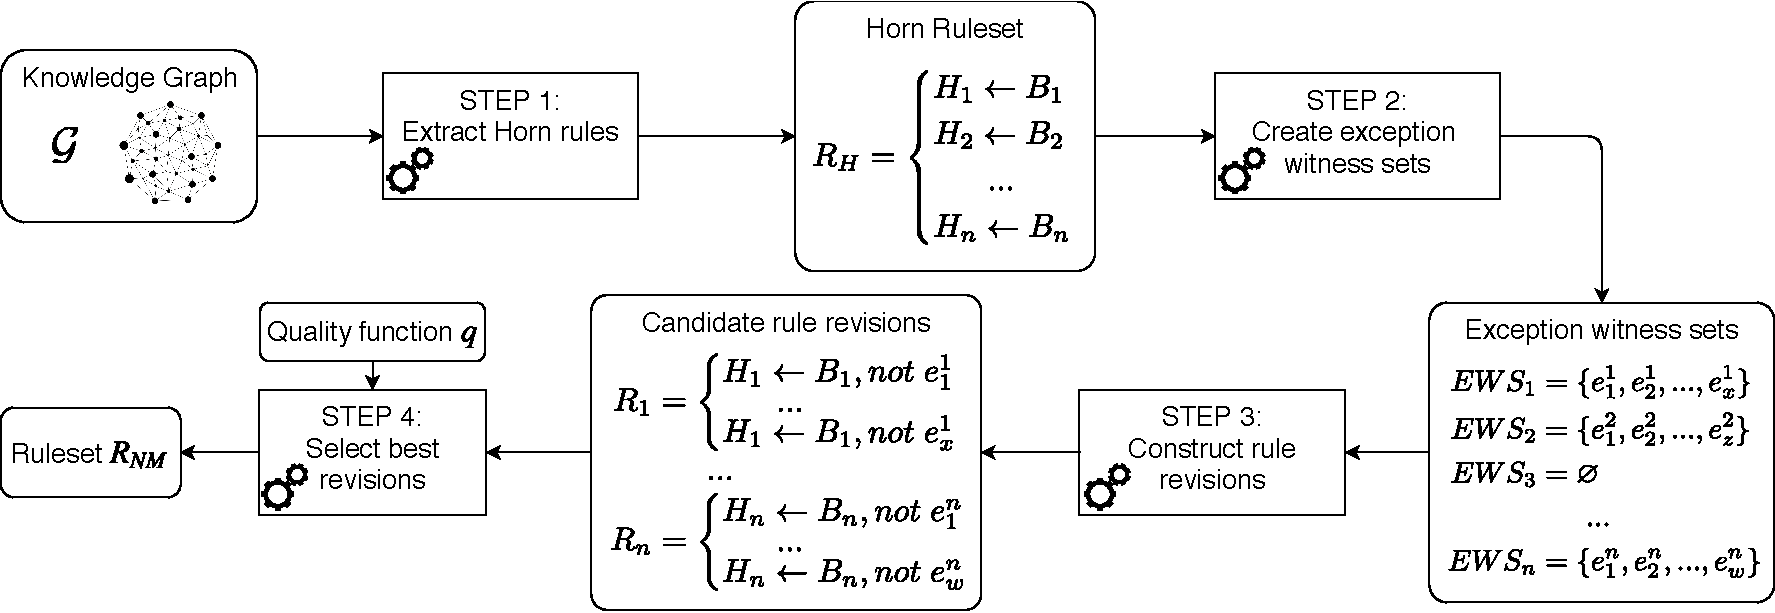
\includegraphics[width=1\textwidth]{figures/overview_new}
\caption{Rule revision method for nonmonotonic rule learning~\cite{gad2016,rumis}.}
\label{fig:iswc_process}
\end{figure}
\noindent \textbf{Step 1.} After mining Horn rules using an off-the-shelf algorithm (e.g.,
 \cite{amie}), %can also be applied)
 one computes for each rule the \emph{normal} and
\emph{abnormal substitutions}, defined as

\begin{definition}[$r$-(Ab)Normal Substitutions]\label{sec:rulelearn}
Let $\cG$ be a KG, $\mi{r}$ a Horn rule mined from $\cG$, and let $\cV$ be a set of variables occurring in $r$. Then
\begin{myitemize}
\item $\mi{NS(r, \cG)=\{\theta\, |\, head(r)\theta,body(r)\theta \subseteq \cG\}}$ is an $\mi{r}$-normal set of substitutions;
\item $\mi{ABS(r, \cG){=}\{\theta'\, |\, body(r)\theta' {\subseteq} \cG\,{,}\,head(r)\theta' {\not \in} \cG\}}$ is an $\mi{r}$-abnormal one, \\
where $\theta,\theta':\cV \rightarrow \cC$.
\end{myitemize} 
\end{definition}

\begin{example}\label{ex:abns}
For $\cG$ from Fig.~\ref{rdf} and $\mi{r1}$ 
we have $\mi{NS(r1,\cG)}=\{\mi{\theta_1,\theta_2,\theta_3}\}$, where $\theta_1=\{\mi{X/brad,Y/ann,Z/berlin}\}$; similarly, $\theta_2=\{\mi{X/john,Y/kate,Z/chicago}\}$ and $\theta_3=\{\mi{X/sui,Y/li,Z/beijing}\}$ resp. Among substitutions in $\mi{ABS(r1,\cG)}$ we have $\theta_4=\{\mi{X/mat,Y/lucy,Z/amsterdam}\}$, yet there are others. \qed 
\end{example}
 

% \begin{example}\label{ex:nab}
% For $\cA$ from Table~\ref{tab:im} and the rule $r:\;\mi{livesInUS(X)}{\leftarrow}\mi{bornInUS(X)}$, $r$-normal and $r$-abnormal instance sets are given as $NS(r,\cA)=\{\mi{p1},\dotsc, \mi{p5}\}$ and $\mi{ABS}(r,\cA)=\{\mi{p6},\dotsc, \mi{p11}\}$ respectively.\qed
% \end{example}

\noindent \textbf{Step 2.} Intuitively, if the given data was complete, then the $r$-normal
and $r$-abnormal substitutions would exactly correspond to instances for which
the rule $r$ holds (resp. does not hold) in the real world. Since the KG is
potentially incomplete, this is no longer the case and some r-abnormal instances
might in fact be classified as such due to data incompleteness.  In order to
distinguish the ``wrongly'' and ``correctly'' classified instances in the
$r$-abnormal set, one constructs \emph{exception witness sets} ($\mi{EWS}$), which
are defined as follows:

%and see whether we
%can find one that can be used to discriminate real  For instance, for $\cA$ from
%Table~\ref{tab:im} a possible reason for abnormality of $\{\mi{p8,p9,p10}\}$
%could be their presence in the predicate $\mi{immigrant}$.


\begin{definition}[Exception Witness Set (EWS)] \label{def:ews}
Let $\cG$ be a KG, let $r$ be a rule mined from it, let $\cV$ be a set of variables occurring in $\mi{r}$ and $\vec{X}\subseteq \cV$. Exception witness set for $r$ \wrt\ $\cG$ and $\vec{X}$ is a maximal set of predicates $\mi{EWS(r,\cG,\vec{X})}=\{e_1,\dotsc,e_k\}$, s.t.
\begin{myitemize}
\item $\mi{e_i}(\vec{X}\theta_j)\in \cG$ for some $\theta_j\in \mi{ABS(r,\cG)}$, $1 \leq i\leq k$ and
\item $\mi{e_1}(\vec{X}\theta'),\dotsc,\mi{e_k}(\vec{X}\theta')\not \in \cG$ for all $\theta' \in \mi{NS(r,\cG)}$.
\end{myitemize}
\end{definition}

\begin{example}
For $\cG$ in Fig.~\ref{rdf} and $\mi{r1}$ 
we have that $\mi{EWS(r,\cG,Y)}=\{\mi{researcher}\}$. Furthermore,
 $\mi{EWS(r,\cG,X)}=\{\mi{artist}\}$. If $\mi{brad}$ with $\mi{ann}$ and $\mi{john}$ with $\mi{kate}$ did not live in %cities different from 
%$\mi{berlin}$ and $\mi{chicago}$ resp., 
metropolitans, then $\mi{EWS(r,\cG,Z)}=\{\mi{metropolitan}\}$. 
\end{example}
In general when binary atoms are allowed in the rules, there might be potentially too many possible $\mi{EWS}$s to construct. 
For a rule with $n$ distinct variables, $n^2$ candidate $\mi{EWS}$s might exist. Furthermore, combinations of exception candidates could be an explanation for some missing links, so the search space of solutions to the above problem is large. In \cite{rumis} a restriction to a single predicate as a final exception has been posed; extensions to arbitrary combinations of atoms is left for future research.



% We illustrate the notion of exception witness candidates by the example.
%Intuitively, $r$-exception witness set explains $r$-abnormality of some instances from $\mi{ABS}(r,\cA)$.

% \begin{example}\label{ex:ews} For $\cA$ and $r$ from Ex.~\ref{ex:nab}
%     $\mi{EWS(r,\cA)}{=}\{\mi{immigrant}\}$ is an $r$-exception witness set. For
%     $\cA'{=}\cA\backslash\{\mi{p5}\}$ it holds that
%     $\mi{EWS(r,\cA')}{=}\{\mi{immigrant,stateless}\}$.\qed \end{example}

\noindent \textbf{Steps 3 and 4.} After $\mi{EWS}$s are computed for all rules in $R_H$, they are used
 to create potential revisions (Step 3), i.e., from every $\mi{e_j}\in \mi{EWS(r_i,\cG)}$ a revision $r^j_i$ of $r_i$ is constructed by adding a negated atom over $\mi{e_j}$ to the body of $r_i$. Finally, a concrete revision for every rule is determined, %that will 
which constitutes a solution to the above problem (Step 4). To find such globally best ruleset revision $R_{\mi{NM}}$ many candidate combinations have to be checked, which due to the large size of %our
 $\cG$ and $\mi{EWS}$s might be too expensive. Thus, instead, $R_{\mi{NM}}$ %it is more reasonable to
is incrementally built by considering every $r_i \in
R_{H}$ and choosing the locally best revision $r^j_i$ %\in R_i$
for it.

In order to select %the following locally-best
$r^j_i$, four special ranking functions are introduced: a naive one and three more advanced functions, which exploit the concept of \emph{partial materialization} (\textbf{\em PM}). Intuitively, the idea behind it is to rank candidate revisions not based on $\cG$, but rather on its extension with predictions produced by other (selectively chosen) rules (grouped into a set $R'$), thus ensuring a cross-talk among the rules. We now describe the ranking functions in more details.

\begin{itemize}
    \item {\textbf{\em Naive}} ranker is the most straightforward ranking function. It prefers the revision $\mi{r^j_i}$ with the highest value of $\mi{rm(r^j_{i},\cG)}$ among all revisions of $r_i$.
    \item {\textbf{\em PM}} ranking function prefers $\mi{r^j_i}$ with the highest value of
\begin{equation}
\label{pm}
\dfrac{\mi{rm(r^j_i,\cG_{R'})+rm({r^j_i}^{aux},\cG_{R'})}}{2}
\end{equation}
 where $R'$ is the set of rules $r_k'$, which are rules from $R_H\backslash r_i$ with all exceptions from $\mi{EWS(r_k,\cG)}$ incorporated at once. Informally, $\cG_{R'}$ contains only facts that can be safely predicted by the rules from $\mi{R_H\backslash r_i}$, i.e., there is no evident reason (candidate exceptions) to neglect their predictions.
%\mi{rm(r^i_j,\cG_{R'\backslash r^i})+rm(r^i_j^{\mi{aux}},\cG_{R'\backslash r^i})}{2}$, where $R'$ is $R_H$ with incorporated exceptions from $\mi{EWS(r_k,\cG)}$ for every $r_k\in R_H$ %TODO
    \item {\textbf{\em OPM}} is similar to \textbf{{\em PM}}, but the selected ruleset $R'$ contains only those rules whose Horn version appears above the considered rule $r_i$ in the ruleset $R_H$, ordered (\textbf{\em O}) based on some chosen measure (e.g., the same as $\mi{rm}$). %TODO
\smallskip

    \item {\textbf{\em OWPM}} is the most advanced ranking function. It differs from \textbf{\em OPM} in that the predicted facts in $\cG_{R'}\backslash \cG$ inherit weights (\textbf{\em W}) from the rules that produced them, and facts in $\cG$ get the highest weight. These weights are taken into account when computing the value of~\ref{pm}. If the same fact is derived by multiple rules,  the highest weight is stored. To avoid propagating uncertainty through rule chaining when computing weighted partial materialization of $\cG$ predicted facts (i.e., derived by applying rules from $R'$) are kept separately from the explicit facts (i.e., those in $\cG$), and %infer 
new facts are inferred using only $\cG$.

For reasoning over weighted facts exiting 
probabilistic deductive reasoning tools such as ProbLog~\cite{problog2007,problog2015} can be used.
\end{itemize}


% \cite{gad2016} and its successor RUMIS~\cite{rumis} have been developed specifically to learn nonmonotonic rules from the large KGs, taking into account the OWA and the huge size of the KG. 
% Both %\cite{gad2016} and RUMIS try to 
% %learn exceptions from a learned rules set % in the KG 
% %by revising % the set of Horn rules $R_H$ extracted from the KG
% % into a nonmonotonic set $R_{MN}$ by
% learn exceptions starting with a learned Horn rules set and revise it by  
% adding at most one negated atom to each rule at a time. The revision is constructed such that the average quality of the Horn rule set is maximized, while the conflict among the predictions of the rules are minimized. To estimate this conflict ratio, the negative predictions are materialized. To this end, % herefore,
% % they introduce 
% the notion of an auxiliary rule for a given rule $r:H \leftarrow B, \naf E$ has been introduced as follows: % , concretely, for a rule 
% %, the auxiliary version is 
% $r^{aux}:\mi{not\_H} \leftarrow B, E$ where $\mi{not\_H}$ is a fresh predicate indicating that $H$ will not be derived by this rule. The number of grounded pairs $\tuple{H,\mi{not\_H}}$ in the answer set generated by the rule set, the auxiliary rules and the KG indicates the degree of conflict.


%Figure shows an overview of the rule revision steps. % 
% In the first step a set of Horn rules is extracted from a KG relying on any existing Horn rule extraction method, such as \cite{amie}.
% In the second step, for every Horn rule the \textit{normal} and \textit{abnormal} substitutions are determined, i.e., substitutions that satisfy (resp. do not satisfy) the considered rule.
% \begin{definition}[(Ab)normal substitutions]
% \begin{itemize}
% \item $NS(r, \cG) = \{\theta \mid head(r)\theta, body(r)\theta \subseteq \cG\}$
% \item $ABS(r, \cG) = \{\theta \mid body(r)\theta \subseteq \cG , head(r)\theta \notin \cG\}$\\
% where $\theta: \mathcal{V} \rightarrow \cC$.
% \end{itemize}
% where $\mathcal{V}$ is the set of variables appearing in $r$. 
% \end{definition}

% Relying on the above notions, the so-called \emph{exception witness sets} are computed, i.e., sets of predicates that are potentially involved in explaining why abnormal substitutions fail to follow the rule. Formally, these are defined as follows:

% \begin{definition}[Exception Witness Set]The Exception Witness Set (EWS) of $r$ with respect to the KG and a variable $X\in V$ is the maximal set of predicates $EWS(r,\cG,\mathcal{X}) = \{p_1,...,p_k\}$ such that:
% \begin{itemize}
% \item $\forall i \in \{1,..,k\} : \exists \theta \in ABS(r, \cG)\ s.t.\ p_i(\mathcal{X}\theta) \in \cG$, and 
% \item $\forall \theta \in NS(r,\cG) :  p_1(\mathcal{X}\theta), ...,p_k(\mathcal{X}\theta) \notin \cG$
% \end{itemize}
% \end{definition}

% Third, candidate rule revisions are constructed by adding to a rule body a single exception at a time. The quality measures for nonmonotonic rules are devised to quantify their strength w.r.t the KG. Importantly, the crosstalk between the rules through is considered via the novel \emph{partial materialization} technique instead of revising rules in isolation. Fourth, the rule revisions are ranked according to these measures to determine a ruleset that not only describes the data well but also shows a good predictive power by taking exceptions into account. 



% \begin{example}
% Consider the KG $\cG$ and $r_1$ from Figure~\ref{rdf} as before, the normal set for $r_1$ is $NS(r_1,\cG)=\{\theta_1, \theta_2 ,\theta_3\}$, where $\theta_1 = \{X/brad, Y/ann, Z/berlin\}$,\\  $\theta_2 = \{X/john, Y/kate, Z/chicago\}$ and $\theta_3 = \{X/sue, Y/li, Z/beijing\}$.\\ and the abnormal set, $ABS(r_1,\cG)=\{\theta_4,\theta_5, \theta_6\}$, \\such that $\theta_4=\{X/bob, Y/alice, Z/berlin\}$,  $\theta_5=\{X/clara, Y/dave, Z/chicago\}$, and $\theta_6=\{X/mat, Y/lucy, Z/amsterdam\}$.
% \qed
% \end{example}



% In the third step the exception witness sets (EWSs) are constructed. 
% \begin{example}
% Recalling $\cG$ and $r_1$, the exceptions witness sets for variables $X$ and $Y$ are $EWS(r_1,\cG,\{X\}) = \{artist\}$ and $EWS(r_1,\cG,\{Y\}) = \{researcher\}$, respectively.
% \qed
% \end{example}
% For each rule $r \in \cR_H$, the EWSs are collected in one set $EWS(r,\cG)$ containing all of its exception candidates. 
% %\[EWS(r,\cG)=\bigcup_{\forall\mathcal{X}\subseteq \mathcal{V}}EWS(r,\cG,\mathcal{X})\] 

% After the exception witness sets are computed for every rule, the search for the best possible revision is performed relying on the following exception scoring functions:
% \begin{itemize}
% \item \textbf{Naive}: Choose the rule revision, with the best standard measure such as confidence or conviction.
% \item \textbf{PM}: Prior to selecting the best revision, apply all other rules that appear in a set with all of their exceptions incorporated. 
% \item \textbf{OPM}: The \textit{ordered partial materialization} is similar to \textbf{PM}, but only materializes the rules from $\cR_{H}$ that are of a higher quality then the given one.
% \item \textbf{OWPM}: The \textit{ordered weighted partial materialization} distinguishes between the original facts in the KG and those predicted by rules by assigning a weight to them, which is inherited from the rules used to generate them. For reasoning over weighted facts exiting % is the concern of 
% probabilistic deductive reasoning tools such as Problog~\cite{problog2007,problog2015} could be used. %or DLV~\cite{dlv2006}.\gad{no sure about DLV citation}
% \end{itemize}



\subsection{Method Guided by Embedding Models}



In the work RulES (rule learning with embedding support)~\cite{thinh2018} an alternative method for nonmonotonic rule induction has been proposed, which first constructs an approximation of an ideal graph $\cG^i$ and then learns rules by relying on it. For building such approximation, representations (i.e. embeddings) of entities and relations are learned from a given KG possibly enriched with additional information sources (e.g., text). We refer the reader to \cite{Wang2017} for an overview of KG embedding models. % -based methods for KG completion.

The RulES approach~\cite{thinh2018} established a framework to benefit from the advantages of these models %while constructing nonmonotonic rule sets 
by iteratively inducing rules from a KG and collecting statistics about them from a precomputed embedding model to prune out not promising rule candidates.
% To explain the core of RulES, l

Let  $\cG$ be a KG over the signature $\Sigma_{\cG}=(\cR,\cC)$.
A \emph{probabilistic KG} is a pair $\cP = (\cG,f)$, 
where $f:\cR\times \cC \times \cC\rightarrow [0,1]$ is a probability function over the facts over $\Sigma_{\cG}$ such that for each atom $a \in \cG $ it holds that $f(a) \geq ct $, where $ct$ is a correctness threshold.

The goal of RulES is to learn rules that not only describe the available graph $\cG$ well, but also predict highly probable facts based on the function $f$ which relies on embeddings of the KG. For that, it utilizes a hybrid rule quality function:
\begin{align*}
	\mu(r,\cP)= (1 - \lambda)\times \mu_1(r,\cG) + \lambda \times \mu_2(\cG_r,\cP).
\end{align*}

\noindent where $\lambda$ is a weight coefficient and $\mu_1$ is any classical quality measure of $r$ over $\cG$ such that $\mu_1: (r,\cG) \mapsto \alpha \in  [0,1]$ (\eg \textit{standard confidence} or \textit{PCA confidence}~\cite{amie}). 
$\mu_2$ measures the quality of $\cG_r$ (\ie the extension of $\cG$ resulting from executing rule $r$) based on $\cP$ such that
 $\mu_2{:}\, (\cG_r,\cP) \mapsto  \alpha \,{\in}\, [0,1]$. To this end, $\mu_2$ is defined as the average probability of the newly predicted facts in $\cG_r$: %, formally defined as:
\begin{align*}
	\mu_2(\cG_r,\cP) = \dfrac{\Sigma_{a\in \cG_r\backslash \cG} f(a)}{|\cG_r \backslash \cG|}.
\end{align*}
  % \gad{Not sure if we should add more here regarding $\mu_2$}



RulES takes as input a KG, possibly a text corpus, and a set of user-specified parameters that are used to terminate rule construction.
These parameters include an embedding weight $\lambda$, 
a minimum threshold 
for $\mu_1$,  
a minimum rule support $\textit{r-supp}$ 
and other \emph{rule-related} parameters such as a maximum number of positive %$\mi{max\_pos}$ 
and negative 
atoms allowed in $\mi{body(r)}$.
The KG and text corpus are used to train the embedding model that in turn is utilized to construct the probabilistic function $f$.
The rules $r$ are computed similar to \cite{amie} in an iterative fashion by applying refinement operators, starting from the head, by adding atoms to its body one after another until at least one of the termination criteria (that depend on $f$) is met. The set of refinement operators from \cite{amie} is extended by the following two to support negations in rule bodies:
\begin{itemize}
\item \emph{add an exception instantiated atom:} add a negated atom with one of its arguments
being a constant, and the other one being a shared variable.
\item \emph{add an exception closing atom:} add a binary negated atom to the rule with both of its
arguments being shared variables or a unary negated atom with a shared variable.
\end{itemize}
 During the construction of a rule $r$, the quality $\mu(r)$ is computed, based on which a decision about the next action is made.


Note that by exploiting the embedding feedback, one can distinguish
exceptions from noise. Consider the rule $r_1$ stating that married people live together. This
rule can have several possible exceptions, e.g., either one of the spouses is a researcher
or he/she works at a company, which has headquarter in the US. Whenever the rule is
enriched with an exception, naturally, the support of its body decreases, i.e., the size of
$\cG_r$ goes down. Ideally, such negated atoms shoudld be added to its body, that the average quality of
$\cG_r$ increases, as this will witness that by adding negated atoms to the rule we get rid of
unlikely predictions.

Figure~\ref{fig:system} demonstrates a high level architecture of RulES, where arrows depict information flow between blocks.
The \emph{Rule Learning} block constructs rules over the input KG similar to rule construction described in Section~\ref{subsec:rule_const}, \emph{Rule Evaluation} supplies it with quality scores $\mu$ for $r$, using $\cG$ and $f$, where $f$ is computed by the \emph{Embedding Model} block from $\cG$ and text. As an output, the system produces a set of nonmonotonic rules suitable for KG completion.



   \begin{figure}[t]
\centering
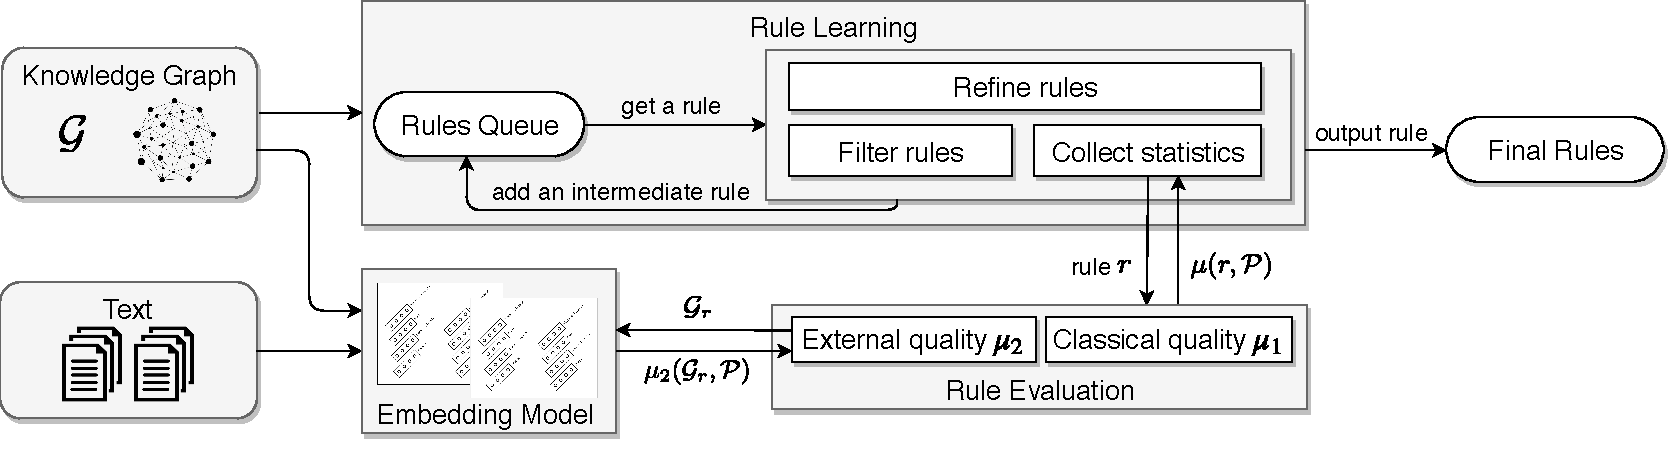
\includegraphics[width=1\textwidth]{figures/rules_overview_H.pdf}
\caption{Embedding-based method for nonmonotonic rule learning.}
\label{fig:system}
\end{figure}

